\subsection{Technische Mittel}
Zum Ausprobieren dieser Verfahren sind ein Ultraschallechoskop, Ultraschallsonden
mit verschiedenen Frequenzen und ein Rechner für die Datenanalyse nötig. Das
Echoskop wird für den Impulsbetrieb verwendent. Mit dem Kippschalter
"REFLEC/TRANS" wird eingestellt, ob das Impuls-Echo-Verfahren oder das
Durchschallungsverfahren benutzt wird. Für letzteres werden zwei gleiche
Ultraschallsonden benötigt. Die Sonden arbeiten in einem Bereich von $0-30 \su{dB}$.
Die Frequenzen betragen $1,2$ und $4 \,\si{\mega\hertz}$. Als Kontaktmittel
wird bidestilliertes Wasser verwendet. Die Auswertung erfolgt mit dem
Programm A-Scan. Im oberen Bereich des Bildschirms kann die Scan-Art gewählt werden.
Bei Verwendung des A-Scans wird mit "Time" eine Funktion der Zeit und mit "Depth"
eine Funktion der Eindringtiefe dargestellt. Für die Berechnung der Eindringtiefe
muss die Schallgeschwindigkeit als Zahlenwert eingegeben werden. Ein Cursor
steht zur Verfügung um Laufzeitdifferenzen und Pulsamplituden zu bestimmen.
Im unteren Bereich des Bildschirms werden Verstärkungen angezeigt (Time Gain
Control). Threshold, Wide, Slope und Start sind verschiedene Verstärkungsparameter.
Mit der FFT-Taste lässt sich ein weiteres Frequenzspektrum anzeigen.
Wird der TM-Mode gewählt, so befindet sich die Messzeit auf der x-Achse und
die Laufzeit auf der y-Achse.

\subsection{Untersuchungen}
Zu Beginn soll der Acrylblock aus Abb. \ref{fig:block} mithilfe eines A-Scans untersucht werden.
\begin{wrapfigure}{r}{6cm}
  \centering
  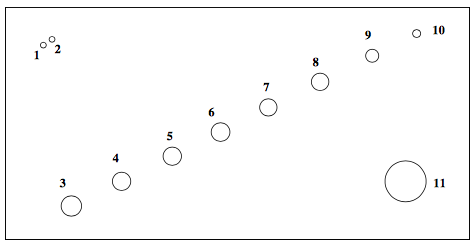
\includegraphics[width=5cm]{bilder/block.png}
  \caption{Acrylblock mit Störstellen \cite{us2}.}
  \label{fig:block}
\end{wrapfigure}
Dazu wird
eine $1 \,\si{\mega\hertz}$ Sonde im Impuls-Echo Betrieb verwendet. Die Schalllaufzeiten
werden an verschiedenen Stellen bestimmt, um die Tiefe der Bohrungen zu bestimmen.
Anschließend wird der Block umgedreht und es wird erneut gemessen. Damit können
Aussagen über die Größe der Löcher getroffen werden. Bei den Laufzeiten muss beachtet werden,
dass die Sonden mit einer Schutzschicht überzogen sind.

Danach wird das Auflösungsvermögen überprüft, indem eine $2 \,\si{\mega\hertz}$
Sonde verwendet wird.. Es wird der gleiche Acrylblock, wie im ersten Aufgabenteil verwendet.

Dann wird der Acrylblock mit einem B-Scan untersucht. Auch hierbei wird eine $2 \,\si{\mega\hertz}$
Sonde verwendet. Die Sonde wird dabei mit konstanter Geschwindigkeit über den Block geführt.
Die Ergebnisse dieses Scans werden dann mit den vorherigen verglichen.

Abschließend wir ein Herzmodell untersucht. Das Modell besteht aus
einem Doppelgefäß mit einer beweglichen Membran, welche mit einem Gummiball periodisch gewölbt werden
kann. Anhand der zurückströmenden Luft kann dann die Herzfrequenz und das Schlagvolumen
bestimmt werden. Es gilt:
\begin{equation}
  HZV = (EDV - ESV)\cdot  \nu_{Herz}
\end{equation}
, mit $\nu_{Herz}$ als Herzfrequenz, $HZV$ als Herzschlagvolumen, $EDV$ als
enddiastolischem Volumen und $ESV$ als endsystolischem Volumen.
$ESV$ beschreibt das Volumen nach maximaler Entleerung des Herzens, $EDV$
beschreibt das Volumen bei maximaler Füllung.
Das Herz wird zu $\sfrac{1}{3}$ mit Wasser befüllt und die Sonde wird so aufgesetzt,
dass sie soeben die Wasseroberfläche berührt. Mit einem A-Scan wird die Laufzeit
bestimmt. Danach wird das Herzvolumen mit dem Ball vergrößert und es soll nachgewiesen
werden, dass der Eingangsimpuls immer noch mit dem A-Scan zu messen ist.
Dann wird zum TM-Mode gewechselt und die Herzfrequenz wird aufgenommen.

Als Kontaktmittel wird Wasser für sämtliche Messungen verwendet.
